\documentclass[10pt,letterpaper]{article} 
%\usepackage{tikz}
%\usepackage{tools}
\usepackage{amsmath,amssymb,geometry,graphicx,enumitem,caption,subcaption}
%\usefonttheme{serif}‎
%\usepackage{ptext}‎
%\usepackage{xepersian}
%\settextfont{B Nazanin}
\usepackage{lipsum}
\setlength{\parindent}{0pt}
\newcommand{\pf}{$\blacksquare$}
\newcommand{\Q}[1]{\textbf{Question #1)}}
\newcommand{\EX}{\Bbb E}
\newcommand{\nl}{\newline\newline}
\providecommand{\pic}[2]{
\begin{center}
\includegraphics[width=#2]{#1}
\end{center}
}
\begin{document}
\Large
\begin{center}
In the name of beauty

The 2nd problem set of Optical Networks course

\hrulefill
\end{center}
\Q1

Determine each of the following statements as either true or false with proper reasoning.

\begin{enumerate}[label=\alph*)]
\item
Load balancing refers to a scheme of layer-3 routing for avoiding overload on a specific server within data centers.
\item
3R-regeneration cleans up signal in an all-optical manner, which makes it economically interesting.
\item
The refractive index of a fiber core should be less than that of its cladding to help trapping light inside the fiber.
\item
Data center networks reside at network core.
\end{enumerate}

\Q2

\begin{enumerate}[label=\alph*.]
\item
Calculate the numerical aperture (NA) for a fiber with a core refractive index of $1.500$ and a cladding refractive index of $1.495$.
\item
How long can a pulse with bit rate equal to 10 Mbit/s propagate through this fiber without suffering modal dispersion?
\end{enumerate}

\Q3

A small section of fiber of length $L$, with 2nd-order disperstion and non-linear coefficient of $\beta_2$ and $\gamma$ can be regarded as a combination of a non-linear operation and a dispersion, linear operation. This means that an input signal $x(t)$ is first multiplied in a non-linear factor $e^{j\gamma L |x(t)|^2}$ and then applied to a linear time-invariant filter $H(j\omega)=e^{j\frac{\beta_2}{2}\omega^2L}$. With $x(t)=e^{j2\pi f_0 t}$, find the output of the fiber section. How much phase rotation is experienced by $x(t)$?
%A link consisting of two equal spans interconnects two nodes as follows:
%\begin{figure}[ht]
%\centering
%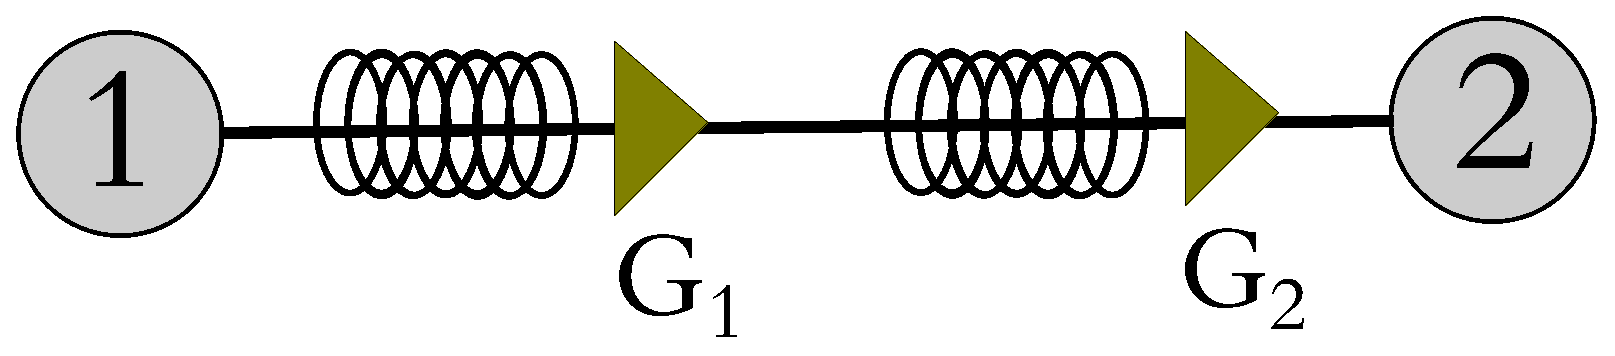
\includegraphics[scale=0.3]{PS2_P2P}
%\end{figure}
%
%Each span is constituted by a single-mode fiber (SMF) of length $L=100\text{km}$ and attenuation coefficient ($\alpha$) of $0.2\text{dB/km}$ and an EDFA. The power gains of the EDFAs are denoted by $G_1$ and $G_2$, the receiver bandwidth is $50\text{GHz}$ and each amplifer has a noise figure of $5\text{dB}$.
%\begin{enumerate}[label=\alph*)]
%\item
%For $G_1=13\text{dB}$ and $G_2=16\text{dB}$, calculate the total noise power at receiver.
%\item
%Assuming the receiver power sensitivity to be $0\text{dBu}$, with $G_1$ and $G_2$ take the same values of part a. Calculate the minimum power that should be launched into the link for a correct detection at receiver (sensitivity is the minimum power that turns on a device on its working point of operation).
%\end{enumerate}
%(Hints: The EDFA noise variance is obtained from
%$$
%\sigma_n^2=h\nu_\text{opt}GFW
%$$
%where
%$h=6.626\times 10^{-34}\text{J.sec}$ and $\nu_\text{opt}=194\text{THz}$. Note that all the scales are linear!
%
%The input power to the receiver is the summation of signal+noise powers.)
%
%\Q4
%
%Assume the same optical system of question 2. The amplifier gain $G_1$ is 10dB, but $G_2$ can arbitrarily vary within (0dB,100dB).
%
%\begin{enumerate}[label=\alph*)]
%\item
%How much is the maximum and minimum of achievable SNR at receiver? Assume the achievable SNR is defined as the ratio of signal power to noise variance at the input of receiver.
%\item
%Which one of either $G_1=10\text{dB},G_2=30\text{dB}$ or $G_1=30\text{dB},G_2=10\text{dB}$ is better from the QoS (quality-of-service) point of view (i.e., leads to more SNR)? What is the general reason of this?
%\end{enumerate}

\end{document}